\section{Tema 1: Fundamentos y propiedades de los fluidos}
\subsection{Hipótesis de medio continuo}
Un fluido se caracteriza por un volumen (V) y una longitud característica (L) donde:

\[L \approx V^{\frac{1}{3}}\]

\begin{figure}[H]
	\centering
	\includegraphics[width=0.5\linewidth]{imagenesTema1/caracteristicasFluido}
	\caption{Magnitudes fundamentales de un fluido.}
	\label{fig:caracteristicasfluido}
\end{figure}
Como el tamaño de una molécula es de $d_0 \approx 10^{-11} \ a \ 10^{-10} m$. Por ello, la longitud característica debe ser mucho mayor que $d_0$ ($L>>d_0$) para así comprender el número suficiente de moléculas y poder estudiar la mecánica de fluidos de manera macroscópica.\\

Además, la longitud debe ser suficiente para que exista equilibrio termodinámico local y así poder aplicar las ecuaciones de estado:

\begin{itemize}
	\item Camino libre medio ($\lambda$) de interacción por choque entre moléculas.
	\begin{itemize}
		\item En líquidos: $\lambda \approx d_o$
		\item En gases: $\lambda >> d_o$
	\end{itemize}
	\[L >> \lambda\]
\end{itemize}

\begin{figure}[H]
	\centering
	\includegraphics[width=0.35\linewidth]{imagenesTema1/caminoLibreMedio}
	\caption{Camino libre medio.}
	\label{fig:caminolibremedio}
\end{figure}

En este fluido, es necesario poder medir:
\begin{enumerate}
	\item \underline{\textbf{Densidad}}: el diferencial de volumen debe ser una muestra significativa a nivel estadístico.
	
	\[\rho(\vec{r},t)=\lim_{{V \to 0}} \frac{\Delta m}{\Delta V}=\frac{dm}{dV} \ \left[{\frac{kg}{m^3}}\right]\] 
	
	
	\begin{itemize}
		\item El fluido es un gas si: $\rho \neq cte \rightarrow \rho=f(\vec{r},t)$
		\item El fluido es un líquido si: $\rho = cte \rightarrow \rho=f(t)$
	\end{itemize}
	
	Si la función depende del tiempo, se dice que está en forma paramétrica.
	
	\begin{itemize}
		\item Peso específico
		\[\gamma=\rho g  \rightarrow g: \text{campo gravitatorio} \left[{\frac{m}{s^2}}\right]\]
		\item Densidad relativa
		\[\rho_{rel}=\frac{\rho}{\rho_{ref}}\]
		
		\begin{itemize}
			\item Líquidos: $\rho_{ref}=\rho_{agua}\approx 10^3 \frac{kg}{m^3}$
				\item Gases: $\rho_{ref}=\rho_{aire_{CN}}\approx 1 \frac{kg}{m^3}$
		\end{itemize}
	\end{itemize}
		
	\item \underline{\textbf{Velocidad}}:
	\[\vec{v}(\vec{r},t)=\lim_{{\Delta V \to 0}} \frac{\sum m_i \vec{v_i}}{\sum m_i} \left[{\frac{m}{s}}\right]\]
	\item \underline{\textbf{Presión}}: Es una magnitud absoluta (siempre mayor que 0):
	
	\[P=\frac{d(\vec{F}\cdot\vec{n})}{dS} =\frac{d{F_n}}{dS} [Pa]\]
	\[1 bar = 10^5 Pa\]
	\[1 atm = 101325 Pa\]
	\[1 mmHg =\rho_{Hg}gh=132.32 Pa\]
	\[1 mca \text{(metros columna agua)} = \rho_{H_2O}gh=9.8\cdot 10^3 Pa\]
	\begin{itemize}
		\item Presión manométrica ($P_{man}$): Se mide normalmente con un manómetro diferencial:
		
		\[P_{man} = P - P_{atm} \rightarrow P>P_{atm}\]
		\item Presión vacuométrica ($P_{vac}$): Se mide normalmente con un vacuómetro.
		
		\[P_{vac}= P_{atm}-P \rightarrow P<P_{atm}\]
		
		\item Presión de vapor ($P_v$): Se refiere al equilibrio de fase líquido - gas. Si la presión es menor que la presión de vapor \textbf{cavita}.
		\item Cavitación: Generación de burbujas en el líquido por estar por debajo de la presión de vapor que posteriormente al subir la presión explotan con violencia. 
	\end{itemize}
	
\end{enumerate}

\subsection{Ecuaciones equilibrio termodinámico local}
En un gas ideal, si las condiciones son subsónicas se cumple que:
\[\frac{P}{\rho}=R_gT \rightarrow R_g\frac{R}{mmr} \rightarrow R ={8.314} \frac{J}{mol K}\]

El fluido está en condiciones subsónicas si:
\[\left| \vec{v}(\vec{r},t) \right|<a=\sqrt {\left. \frac{\partial P}{\partial \rho} \right|}_{S=cte}\]

\begin{itemize}
	\item Ecuación isoentrópica: Procesos rápidos.
	\[PV^\alpha=cte\]
	\item Ecuación isoterma: Procesos lentos.
	\[PV=cte\]
\end{itemize}
\subsection{Fuerzas y respuestas en sólidos y fluidos}
\begin{enumerate}
	\item \underline{\textbf{Fuerzas en un fluido}}:
	\[F=f(\Delta \dot{x})=C\dot{x} \rightarrow C: \text{constante de amortiguamiento}\]
	
	\item \underline{\textbf{Tensión tangencial o de cizalladura}}($\tau$):
	\[\tau=\lim_{{S \to 0}} \frac{\Delta F_t}{\Delta S}=\frac{dF_t}{dS}\]
	\item \underline{\textbf{Viscosidad}}($\mu$):
	En fluidos newtonianos la viscosidad es relativamente constante: 
	\[\mu=f(T) [Pa \cdot s]\]
	\[\tau =\mu \dot{\varepsilon} = \mu \frac{\Delta v_n}{\Delta l_n} \rightarrow \dot{\varepsilon}\ \text{es la velocidad de deformación} [s^-1]\]
\begin{figure}[H]
	\centering
	\includegraphics[width=0.7\linewidth]{imagenesTema1/viscosidad}
	\caption{Cálculo de viscosidad.}
	\label{fig:viscosidad}
\end{figure}

\[\tau =\frac{F}{A}=\mu \frac{\Delta v_n}{\Delta l_n} =\mu \frac{v - 0}{l_n}= \mu \frac{v}{l_n}\]
	 
	 En fluidos no newtonianos la viscosidad no es constante:
	 
	 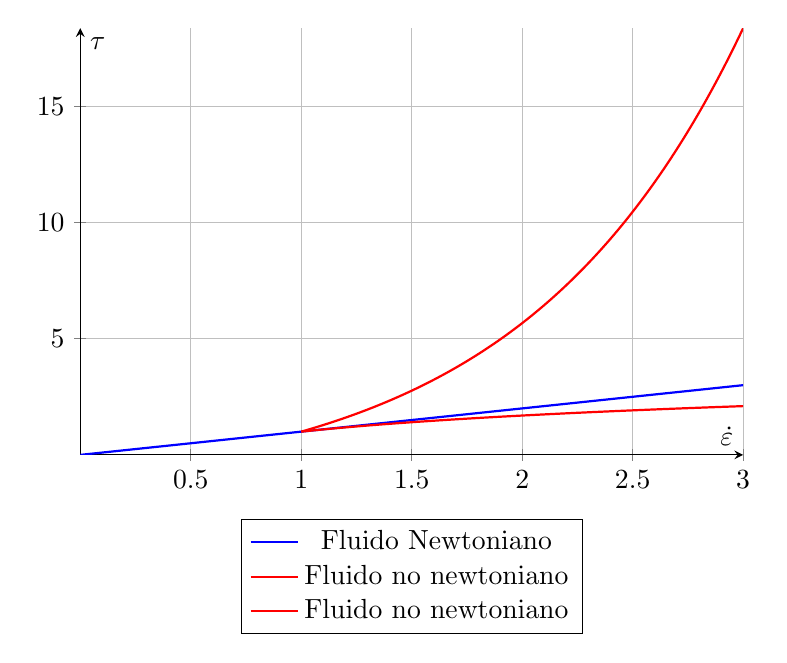
\begin{tikzpicture}
	 	\begin{axis}[
	 		domain=0:3,
	 		samples=100,
	 		height=7cm,
	 		width=10cm,
	 		title={},
	 		ylabel=$\boldsymbol\tau$,
	 		xlabel=$\dot{\boldsymbol\varepsilon}$,
	 		grid=major,
	 		axis lines=center,
	 		legend style={at={(0.5,-0.15)}, anchor=north},
	 		]
	 		\addplot[blue, thick] {x};
	 		\legend{Fluido Newtoniano}
	 		
	 		\addplot[red, thick, domain=1:3] {ln(x)+1};
	 		\addlegendentry{Fluido no newtoniano}
	 		
	 		\addplot[red, thick, domain=1:3] {e^x-e^1+1};
	 		\addlegendentry{Fluido no newtoniano}
	 	\end{axis}
	 \end{tikzpicture}
	 
	 Viscosidades típicas:
	 \[\mu_{H_2O}=10^{-3} Pa \cdot s = 1cP \rightarrow P \ \text{Poise}\]
	
	\item \underline{\textbf{Viscosidad cinemática}}:
	
	\[\nu = \frac{\mu}{\rho} \left[\frac{m^2}{s}\right] \rightarrow 1 csk = 10^{-6}\left[\frac{m^2}{s}\right] \rightarrow csk \ \text{centi-stoke}\]
	
	\item \underline{\textbf{Interfases}}: 
	\begin{itemize}
		\item Vaso grande: Existe intercambio de moléculas en la interfase pero las presiones se equilibran.
		 \begin{figure}[H]
		 	\centering
		 	\includegraphics[width=0.5\linewidth]{imagenesTema1/vasoGrande}
		 	\caption{Interfase Vaso grande.}
		 	\label{fig:vasogrande}
		 \end{figure}
		 
		\item Vaso pequeño: Existe efecto de la tensión superficial ($\sigma \left[
		\frac{N}{m}\right]$) descrita mediante la ecuación de Laplace-Young. Solo aplica a fluidos inmiscibles. 
		\begin{figure}[H]
			\begin{minipage}{0.7\textwidth}
				\centering
				\includegraphics[width=0.2\linewidth]{imagenesTema1/vasoPeque}
				\caption{Efecto tensión superficial Vaso pequeño}
				\label{fig:vasopeque}
			\end{minipage}%
			\begin{minipage}{0.3\textwidth}
				\[P_a - P_{liquido}=\sigma K\]
			\[K \ \text{expresión de la curvatura}\]
			\[K=\nabla_s \vec{n} = \left(\frac{1}{R_i}+\frac{1}{R_j}\right) \]
			\[R_i \ y \  R_j \ \text{son radios característicos}\]
			
			\end{minipage}
		\end{figure}

		\item Zona de efecto: La tensión superficial siempre presenta efectos, no obstante solo se aprecia en una región concreta.
		\[\rho g l_c \approx \sigma \rightarrow l_c \approx \left(\frac{\sigma}{\rho g}\right)^{\frac{1}{2}}\]
		
		\begin{figure}[H]
			\centering
			\includegraphics[width=0.4\linewidth]{imagenesTema1/zonaEfectos}
			\caption{Zona de efecto.}
			\label{fig:zonaefectos}
		\end{figure}
		
		\item Casos particulares
		\begin{enumerate}
			\item Chorro
			\begin{figure}[H]
				\begin{minipage}{0.4\textwidth}
				\centering
				\includegraphics[width=0.7\linewidth]{imagenesTema1/chorro}
				\caption{Chorro.}
				\label{fig:chorro}
			\end{minipage}%
			\begin{minipage}{0.3\textwidth}
			\[P_i - P_e =\sigma\left(\frac{1}{R_i}+\frac{1}{R_j}\right)=\frac{\sigma}{R}\]
			
			\end{minipage}
			\end{figure}
			
			\item Gota
			
			\begin{figure}[H]
				\begin{minipage}{0.4\textwidth}
				\centering
				\includegraphics[width=0.7\linewidth]{imagenesTema1/gota}
				\caption{Gota.}
				\label{fig:gota}
					\end{minipage}%
				\begin{minipage}{0.3\textwidth}
				\[P_i - P_e =\sigma\left(\frac{1}{R_i}+\frac{1}{R_j}\right)=\frac{2\sigma}{R}\]
				
				\end{minipage}
				
			\end{figure}
			
			\item Pompa
			
			\begin{figure}[H]
				\begin{minipage}{0.4\textwidth}
				\centering
				\includegraphics[width=0.7\linewidth]{imagenesTema1/pompa}
				\caption{Pompa.}
				\label{fig:pompa}
			\end{minipage}%
			\begin{minipage}{0.3\textwidth}
			\[P_i - P_m =\frac{2\sigma}{R}\]
			\[P_m - P_e =\frac{2\sigma}{R}\]
			\[P_i - P_e =\frac{4\sigma}{R}\]
			
			\end{minipage}
			\end{figure}
			
			\item Plano
			
			\begin{figure}[H]
								\begin{minipage}{0.4\textwidth}
				\centering
				\includegraphics[width=0.7\linewidth]{imagenesTema1/plano}
				\caption{Plano.}
				\label{fig:plano}
			\end{minipage}%
			\begin{minipage}{0.3\textwidth}
			\[P_i - P_e =\sigma\left(\frac{1}{R_i}+\frac{1}{R_j}\right)=0\rightarrow P_i = P_e\]
			
			\end{minipage}
			\end{figure}
			
		\end{enumerate}
	\end{itemize}
\end{enumerate}

\subsection{Mojabilidad}
\begin{itemize}
	\item Un líquido no moja a un sólido si $\theta_c \gtrsim \ang{150} $. Sólido hidrofóbico.
	\item Un líquido moja a un sólido si $\theta_c  \lesssim \ang{45}$. Sólido hidrofílico totalmente.
\end{itemize}
\begin{figure}[H]
	\centering
	\includegraphics[width=0.7\linewidth]{imagenesTema1/mojabilidad}
	\caption{Mojabilidad.}
	\label{fig:mojabilidad}
\end{figure}
